\documentclass[conference,compsoc]{IEEEtran}

\usepackage{hyperref}
\usepackage{graphicx}	% For figure environment
\usepackage{fancyhdr}
\usepackage{subcaption}
\usepackage{wrapfig}
\usepackage{amsmath}
\usepackage{amsfonts}
% algorithms
\usepackage{algorithm}
\usepackage{algorithmic}
\usepackage[algo2e]{algorithm2e}
\usepackage{verbatim}
\usepackage{xspace} % for algorithm names
\pagestyle{fancy}

\lhead{Markov Chains and Algorithmic Applications}
\rhead{
\includegraphics[width=1cm]{images/EPFL.png}}

\newcommand{\selected}{\mathcal{S}}
\newcommand{\newselected}{\hat{\mathcal{S}}}

\DeclareMathOperator*{\argmax}{arg\,max}
\DeclareMathOperator*{\argmin}{arg\,min}

%%%%%%%%%%%%%%%%%%%%%%%%%
%%%%%% COMMENTING
%%%%%%%%%%%%%%%%%%%%%%%%%
% % when preparing version to submit, fix below...: %
% \setlength{\marginparwidth}{5cm} %
% \usepackage[cam,width=30truecm,height=28truecm,center]{crop}
% \usepackage[textwidth=2cm]{todonotes}

% \providecommand{\mycomment}[3]{\todo[caption={},size=footnotesize,color=#1!20]{\textbf{#2:
% }#3}}% \providecommand{\inlinecomment}[3]{% {\color{#1}#2: #3}}%
% \newcommand\commenter[2]%
% {%
%   \expandafter\newcommand\csname i#1\endcsname[1]{\inlinecomment{#2}{#1}{##1}}
%   \expandafter\newcommand\csname #1\endcsname[1]{\mycomment{#2}{#1}{##1}}
% }

% \commenter{delio}{red} \commenter{ahmad}{purple} \commenter{heloise}{green}
% \setlength{\marginparwidth}{1.5cm}
% %%%%%%%%%%%%%%%%%%%%%
% %%%% remove the above lines for submission

% %%%%%%%%%%%%%%%%%%%%%
\begin{document}
\title{\Large Mini-project : Deploying a 5G Network in a country }

\vspace{- 50 px}

\author{Delio \textsc{Vicini}, Ahmad \textsc{Ajalloeian} and Heloise
\textsc{Dupont de Dinechin} (Team name: DHA)\\
}

\maketitle
\begin{abstract}
  In this project, we use the Metropolis algorithm to optimize a complex
  geometric objective function. The objective function is motivated by the
  problem of optimally placing 5G antennas on a given map of cities. We would
  like to cover cities according to a per city value, while at the same time
  minimizing the spatial spread of the network. We show how to efficiently
  optimize the given objective function, making use of the geometric properties
  of the problem to implement a method which scales favorably in the number of
  considered cities.
\end{abstract}

\section{Introduction}
Given a map of cities, we would like to establish a network of 5G antennas. Due
to constraints on the availability of a maintenance team, the network of
antennas initially should be established in a localized region. The goal is to
cover a significant portion of the cities, while not increasing the distance
traveled by maintenance workers too much. Formally, the problem has been
specified as a maximization of the objective function:
\begin{align}
    f(\lambda, \selected) = \sum_{i \in \selected} v_i - \lambda \cdot n \cdot \max_{(i, j) \in \selected} \pi (d(x_i, x_j) /2) ^2
    \label{eq:objective}
\end{align}

In practice, we will work on the following non-convex minimization objective:

\begin{align}
    f(\lambda, \selected) = -\sum_{i \in \selected} v_i + \lambda \cdot n \cdot \max_{(i, j) \in \selected} \pi (d(x_i, x_j) /2) ^2
    \label{eq:objective}
\end{align}
where $v_i$ are the (normalized) population values associated to each city,
$x_i$ their 2D position, $\lambda$ a scalar and $n$ the total number of cities.
The distance $d(x_i, x_j)$ is the euclidean distance between the cities $i, j$,
and the set $\selected$ is a selected subset of all cities.



\begin{wrapfigure}{R}{0.25\textwidth}
\vspace{-10pt}
%\centering
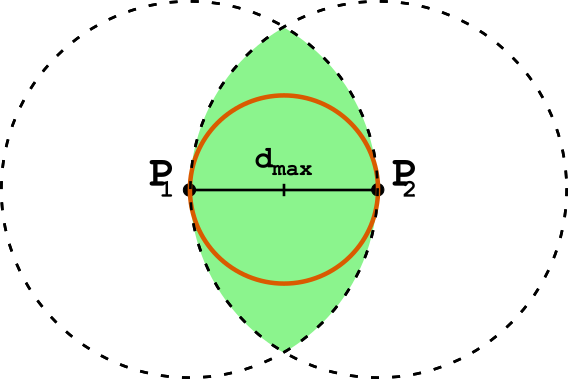
\includegraphics[width=0.25\textwidth]{images/path899.png}
\vspace{-15pt}
\caption{}
\vspace{-15pt}
\label{fig:zones}
\end{wrapfigure}
A naive bruteforce strategy to optimize this objective function would be to try
out all $2^n$ possible selections $\selected$ of all cities. This quickly
becomes computationally intractable.



Another bruteforce approach would be to iterate over all pairs of cities (in
$O(n^2)$). For each pair of cities, we then assume that the maximum pairwise
distance of the selected cities $\selected$ is attained by this particular pair.
In other words, we assume that given the cities with the maximum distance, there
has to be a single optimal selection $\selected$. We could then try to add
further cities, as long as they do not change the maximum distance value. As
seen in Fig \ref{fig:zones}, if $p_1$ and $p_2$ are the two points attaining the
maximum distance, all further selected points need to be inside the green zone,
while having a maximum distance between them smaller than the distance between
$p_1$ and $p_2$. A reasonable way to do this would be to create a circle with
the radius set to half the maximum distance between the originally selected pair
of cities, centered at their midpoint, the red circle in Fig \ref{fig:zones}.
All cities within that circle can then be added to the selection without
increasing the maximum distance. This however is \emph{not} optimal, as
potentially some cities outside the circle could be added without increasing the
maximum distance. In short, such a strategy would not reliably find the optimal
solution, and it's complexity would still be on the order of $O(n^3)$.\

Therefore, we use the Metropolis algorithm \cite{metropolis53} to optimize the
given objective function. Using Metropolis, we can solve this problem for very
large numbers of cities (up to 100,000 without any issues). In the following, we
first describe how a naive implementation of Metropolis would solve the problem.
We then improve over this baseline by using the geometric properties of the
objective function. We further make use of geometrical algorithms to reduce the
computational complexity of our Metropolis-Hastings implementation.


\section{Method}
\label{sec:method}

\subsection{Problem statement}
Given the non-convex, discrete nature of the optimization problem in
Equation~\ref{eq:objective}, Metropolis seems to be a good choice to optimize
$f$. Our goal is to find the selection $\selected^*$ of cities such that
\begin{align}
    \selected^* = \argmin_{\selected} f(\lambda, \selected)
\end{align}
The parameter $\lambda$ is assumed to be fixed and is part of the problem
specification. The Metropolis algorithm now works as follows: we start from an
initial selection $\selected$. In each iteration, we then randomly sample a new
state $\newselected$. The new state is then accepted with probablity:
\begin{align}
    a = \min \left[1, \exp(-\beta (f(\lambda, \newselected) - f(\lambda, \selected))) \right]
\end{align}
where $\beta$ a positive constant also called the \emph{inverse temperature}.
This acceptance probablity formulation implies that whenever the new loss value
is lower than the previous one, the new state is accepted. If the new loss value
is larger than the old one, the state might be accepted, but that depends on
$\beta$ and the amount the loss increases. A small value of $\beta$ will make it
more likely that non-improving states are accepted. Accepting states which do
not decrease the loss function is important to escape local minima, but can also
lead to a poor final solution if $\beta$ is too small. If $\beta$ is 0, the
solution space is explored randomly without considering the optimization
objective at all. If $\beta$ is infinite, we will only ever accept solutions
which decrease the loss function. In the following we now describe different
ways in which the Metropolis algorithm can be applied to our problem.

\subsection{Strategies}
\label{subsec: strategies}
%\paragraph{Baseline}
\subsubsection{Baseline}
The simplest application of the Metropolis algorithm just randomly selects and
deselects one city in each iteration. We start with no cities selected, i.e.
$\selected = \lbrace \rbrace$. In each optimization iteration, we uniformly
sample an index $k \in \lbrace 1, ..., n \rbrace$. If the city $k$ is in the
current selection $\selected$, we remove it. If it's not in the current
selection, we add it $\selected = \selected \cup \lbrace k \rbrace$. In each
case we then accept this change with the acceptance probability. This is similar
to the flipping strategy usually used in the Ising model spin assignment
\cite{newman1999monte}. This simple strategy indeed works and finds some local
optimum to $f$. However, we found that this strategy also has some limitations.
By randomly adding and removing individual cities, the algorithm struggles to
efficiently explore the whole space of possible solutions. Regardless of how
$\beta$ is set, it seems that the final result of this method highly depends on
the random seed: indeed, once a lot of cities from the same area have been
added, it will struggle to jump to a solution where the cities selected are in a
completely different place. As $n$ becomes larger (e.g. $n=1000$), another issue
occurs: if $\lambda$ is small enough that the optimal solution should select a
significant fraction of all cities, it takes a lot of steps to add them and this
first strategy does not perform well.

\subsubsection{Convex hull}
The objective function that is used implies some very geometric constraints.
Indeed, the maximum distance term requires the computation of the
\textit{diameter of a point set}. A naive computation of this diameter would be
in $O(n^2)$, but it turns out that it can be easily computed using the convex
hull, see \cite{diameter}. The maximum pairwise distance of a set of points is
equal to the maximum pairwise distance of vertices on their convex hull. This
means in particular that at each step we can safely add all the cities that lie
inside the convex hull of the already selected cities. This idea can be used to
improve the complexity of our baseline algorithm, but it also leads to another
strategy. In this one, at each step we chose to compute the objective function
as if all the points contained in the convex hull of the current selection had
been added, without truly adding them. This allows to more efficiently cover
larger regions of the map, especially if the number of cities is large. Note
that for all our methods, we add all the points in the convex hull at the end of
the optimization, as this can only improve the result.

% \begin{wrapfigure}{R}{0.25\textwidth} \vspace{-10pt} %\centering
% 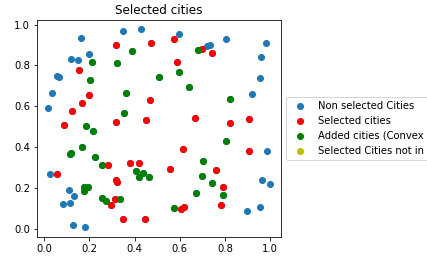
\includegraphics[width=0.25\textwidth]{images/conve_hull.png} \vspace{-15pt}
% \caption{} \vspace{-15pt} \label{fig:zones} \end{wrapfigure}

\subsubsection{Clustering} As described, the drawback of the baseline method is
that it is very inefficient when there are many cities. One solution is to
approach the problem hierarchically. Clustering can be used: the optimization
can be done over 10 mega-cities, then 100, ..., to N cities, using $\log_{10}N$
clustering steps. We implemented a very simple version of such an algorithm.
This method first solves the optimization on the 10 most populated cities, then
uses that result to initialize the solver for the 100 most populated cities,
etc. This works reasonably well, but also has failure cases, as we will discuss
later.

%\paragraph{Continuous Markov Chain}
\subsubsection{Continuous Markov Chain}
We found that solution strategies based on directly modifying a discrete set of
selected cities inherently struggle to use the geometrical properties of the
problem. Once they selected a cluster of cities in one region, they tend to
mostly stick to it and not be able to drastically change it. We noticed that the
distance term in the loss function strongly favors solutions which select all
cities in a mostly circular region. While there is no guarantee that the best
solution lies in a circle, it intuitively makes sense to try different circular
selections of cities. Therefore, we decided to build a solution which explores
the solution space by running the Metropolis algorithm on the parameters of a
circle. We then consider all the cities inside this circle as our current
selection. Formally, the parameters of our Markov chain are now a circle center
$c \in \mathbb{R}^2$ and radius $r > 0$. At each iteration, we either modify the
radius or the circle center, with a 50\% chance each. For the center, we compute
the new center as $\hat{c} = c + u$, with $u \sim \mathcal{N}_2(0, 0.04)$. To
improve global exploration, we occasionally do a larger mutation with $u \sim
\mathcal{N}_2(0, 0.2)$. The probability for a large mutation is 0.05. If we
decide to modify the radius, we compute the new radius as $\hat{r} = \max(0.01,
r + v)$ with $v \sim \mathcal{N}(0, r / 10)$. The change in the circle radius is
proportional to the current radius. We found these parameters to work well, but
we did not tune them systematically, as the method did not seem very sensitive
to these. To compute the acceptance probablity, we then find all the cities
inside the given circle and compute the original loss function using this set of
current cities. Note that the proportional change of the radius makes the
underlying Markov Chain non-symmetrical, but we did not find this to be an issue
in practice. This continuous formulation reliably outperforms all our other
strategies.

% \subsection{Beta} \textit{(draf)} important parameter beta. \textit{simulated
% annealing} is interesting : start with beta small, then increase beta. This
% tuning of beta wouldn't work so well on the baseline strategy: once cities
% have been added, it can be hard to remove them. If we start with a small beta,
% we would tend to a situation where 50\% cities are selected ; we have seen
% that then this state is a very bad initialization step for the rest, will end
% up adding a large number of cities, won't be able to find solution where only
% few cities should be selected.

% But it can work well in other strategies: clustering and smooth


\section{Implementation}
We implemented our method and baselines using Python, relying heavily on Numpy
\cite{harris2020array} and Scipy \cite{scipy} for efficiency. The objective
function evaluation is completely vectorized, as our initial unvectorized
implementation using Python for-loops was very slow (on the order of minutes of
computation for $n=100$ and 1000 iterations). Our final implementation runs on
the order of seconds for small problem sizes ($n \leq 10,000$) and in around 30
seconds to 1 minute on $n = 100,000$ (measured on an AMD Ryzen 5 3600 CPU). The
timings depend on the setting for $\lambda$. The lower $\lambda$, the more
cities have to be selected and the more costly the iterations become. We run our
method for 5000 to 10000 iterations, which seems to be sufficient for
convergence. In the following we briefly discuss some of the implementation
details.

\subsection{Loss function}
The run time of the algorithm is largely determined by the performance of
evaluating the loss function $f$ for the current state of the Markov chain. In
each iteration of the algorithm, we need to evaluate the loss function to
compute the acceptance probability. Computing the mutation itself is typically
very cheap.

To lower the cost of evaluating the cost function, we only evaluate it once per
iteration and keep track of the loss value of the previous state. Further, the
main cost of evaluation the function $f$ comes from the distance term. The sum
of the values of the cities is trivial to compute in $O(n)$, and potentially
could even be computed in $O(1)$ if the previous sum of $v_i$ terms is stored
after each iteration.

The costly term in the loss function is the maximum of the pairwise squared
euclidean distances. A naive implementation of this computation has cost
$O(n^2)$. When adding a single city to an existing selection, we could recompute
the maximum distance in $O(n)$ by evaluating the distance of the newly added
cities to all previous cities, if we assume that we know the previous maximum
distance. However, we will not be able to do the same simplification if we
decide to remove a city. Then we will again have to recompute all pairwise
distances. Fortunately, the distance term can be computed as the maximum
pairwise distance of the vertices of the convex hull of the current selection.
The complexity of the convex hull computation is in $O(n \log n)$ or $O(n \log
h)$, where $h$ is the number of vertices in the convex hull. We use Scipy's
implementation of the convex hull algorithm. Using this optimization gave a
significant performance improvement compared to the naive maximum distance
computation.

\subsection{Cities inside a circle}
When using our continuous formulation, we do not only need to evaluate the loss
function, but we also need to determine which cities are inside the current
circle. We do this using the KD-tree implementation in Scipy. The KD-tree allows
for an efficient query of all points in a circle. We found this to improve
performance for larger number of cities ($n > 10000$). For a small number of
cities, a naive implementation is not much slower.


\subsection{Beta Parameter}
We found the process of tuning the parameter $\beta$ to reach the best (fixed)
parameter not effective. In practice there was not any significant difference
over different choices of $\beta$ and there was a large standard deviation in
the final loss value when running for different initializations of a fixed
$\beta$ regime. We found that in practice increasing the $\beta$ from small to
large values during the optimization process is more effective, a process which
is called \textit{simulated annealing}. By starting with a small $\beta$, the
algorithm visits all the states almost uniformly in the beginning. After a
sufficient number of iterations, we can increase the $\beta$ and run the
algorithm again from the state found from the previous step. We can redo this
process multiple times and gradually increase $\beta$ until we are almost sure
that we have reached the global minimum with high probability. Algorithm
\ref{algo: simulated annealing} shows the simulated annealing process we used in
our experiments.
\begin{algorithm}[htb]
   \caption{Simulated annealing}
   \label{algo: simulated annealing}
\begin{algorithmic}
   \STATE {\bfseries Input:} total number of iterations $n$, current iteation
   $i$ \IF{$i < \frac{n}{5}$} \STATE {$\beta = 1$} \ELSIF{$i < \frac{2n}{5}$}
   \STATE{$\beta = 5$} \ELSIF{$i < \frac{3n}{5}$} \STATE{$\beta = 10$} \ELSIF{$i
   < \frac{4n}{5}$} \STATE{$\beta = 20$} \ELSE \STATE{$\beta = 50$}\ENDIF \STATE
   {\bfseries Return:} $\beta$
\end{algorithmic}
\end{algorithm}

\subsection{Parallelization}
%\paragraph{Parallelization}
Lastly, we found that even using our continuous implementation, different random
seeds do not always converge to the same optimal result. It is therefore still
advantageous to run the optimization several times with different random seeds.
Among all these runs, we can then pick the result with the lowest error. In
practice, we can easily parallelize the algorithm over different random
initializations. This means that running different random seeds is not very
costly, as most modern systems can run at least 8 threads simultaneously. We
implemented this parallel execution using Python's \emph{multiprocessing} module
and built-in thread pool.

\section{Results}
\label{sec:results}

\subsection{Comparison between strategies}


\begin{figure}
    \centering
    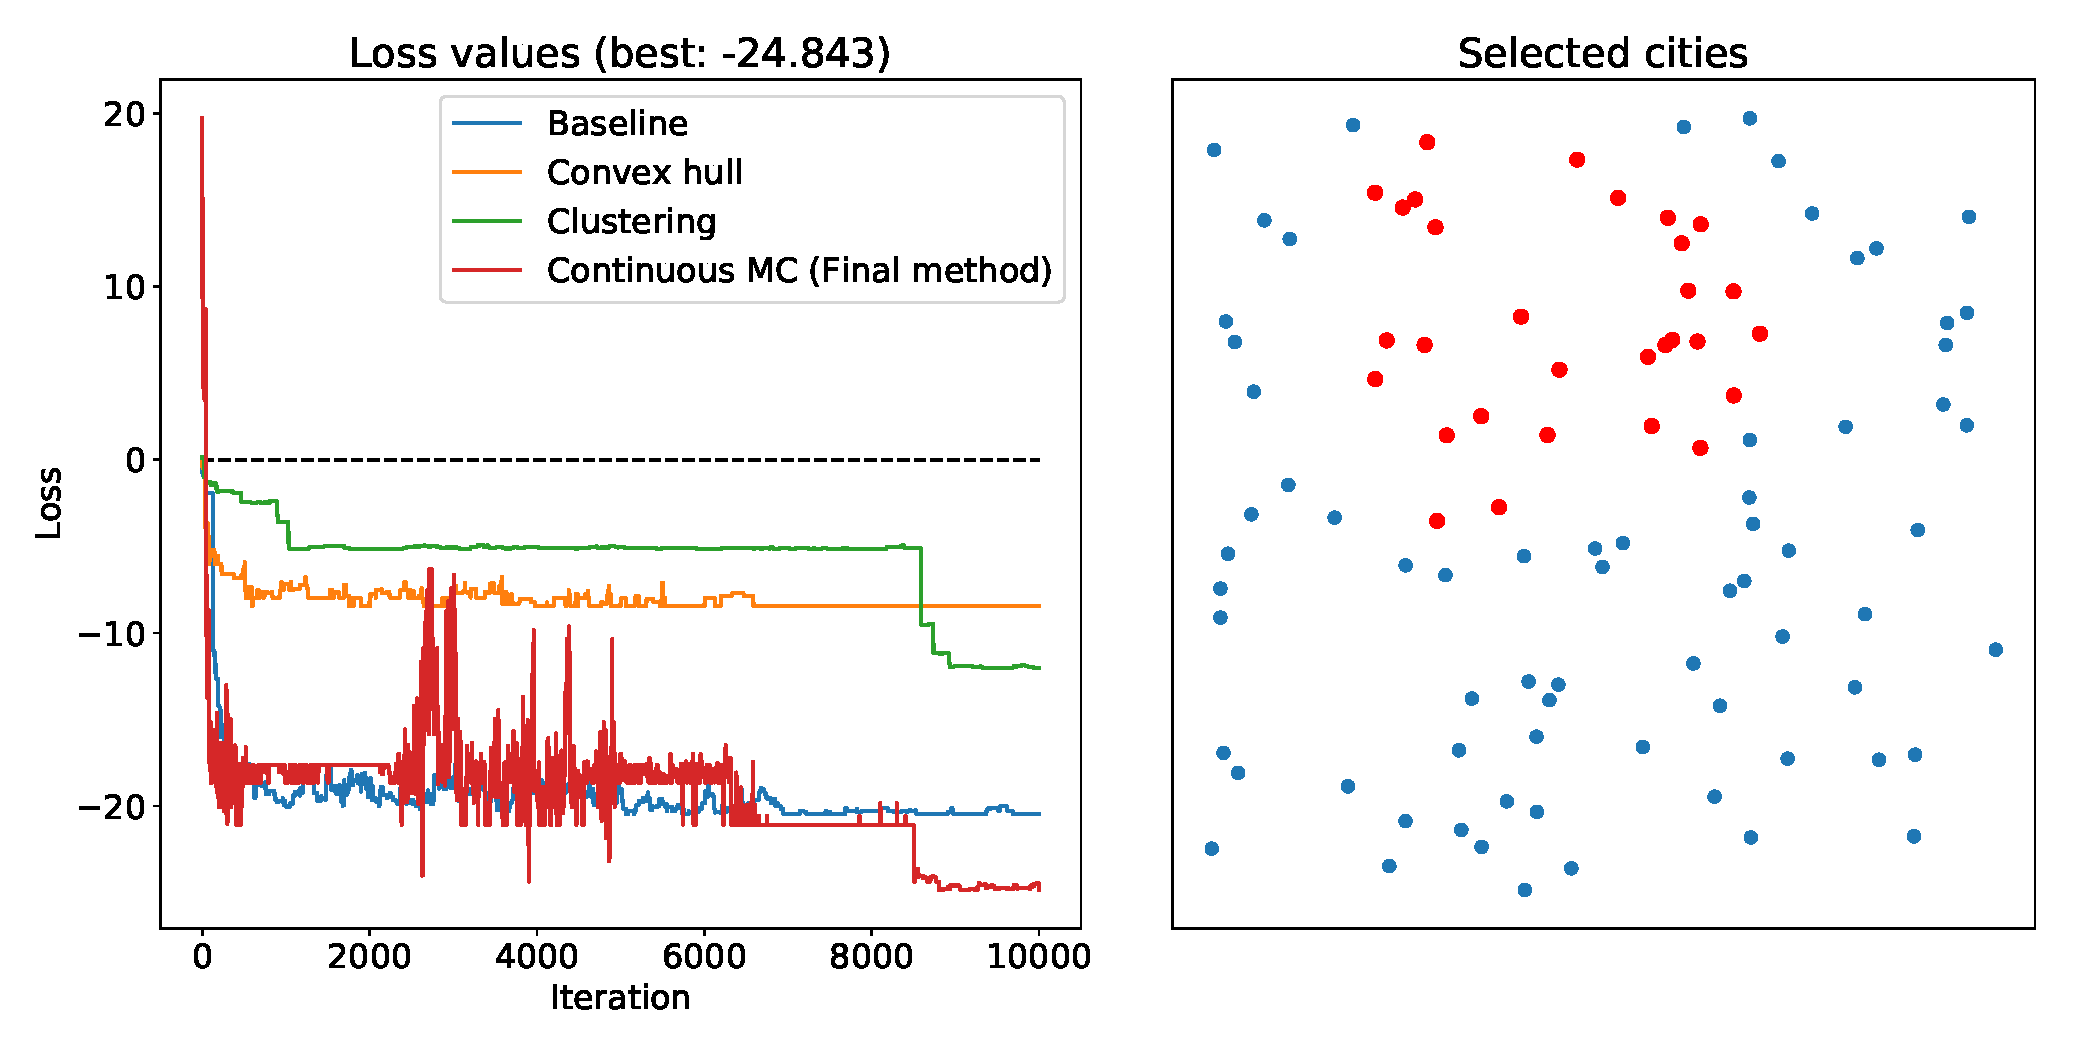
\includegraphics[width=\columnwidth,height=0.5\columnwidth]{images/selected_cities_plot.pdf}
    \caption{Plots of optimization losses over iterations for all our techniques and visualization of the map of cities and the final solution found by our algorithm (selected cities in red)}
    \label{fig:selection}
\end{figure}

The baseline is quite slow and inefficient for large set of cities: in this
case, the loss of the obtained solution is often greater than zero, meaning that
it is worse than selecting a single city. This is improved by using en empty set
as the initialization state and a high beta, but it is not enough. The
\textit{convex hull} method performs well in certain cases, in particular when
the number of cities is large ($ n \geq 1000$). The clustering methods can give
pretty good solutions when a large number of cities are the solution (small
$\lambda$), but at a cost of performance: our simple implementation does not
really scale beyond 1000 cities. Overall, continuous Markov chain strategy
provides the best results and scales up to 100,000 cities without any issues.

We ran experiments on two different distribution of the cities' populations and
for different values of $\lambda$. We mainly used the uniform distribution
$\mathcal{G}_1$:
\begin{align*}
    \mathcal{G}_1^n &: \lbrace (v_i)_{1\leq i \leq n} \sim \mathcal{U}([0, 1]),  (x_i)_{1\leq i \leq n} \sim \mathcal{U}([0, 1]^2) \rbrace
\end{align*}
and the log-normal distribution $\mathcal{G}_2$:
\begin{align*}
    \mathcal{G}_2^n &: \lbrace (\ln v_i)_{1\leq i \leq n} \sim \mathcal{N}(-0.85, 1.3),  (x_i)_{1\leq i \leq n} \sim \mathcal{U}([0, 1]^2)\rbrace
\end{align*}

We ran the Metropolis algorithm with the strategies introduced in Section
\ref{subsec: strategies} to optimize the equation \eqref{eq:objective} for both
of the distributions $\mathcal{G}_1$ and $\mathcal{G}_2$.
Figure~\ref{fig:selection} shows the convergence plots for the different
algorithms run on an example data set with distribution $\mathcal{G}_2$ and $n =
100$. Figures \ref{fig:loss_plots100} and \ref{fig:loss_plots} show a comparison between our different strategies over different choices of $\lambda$ for the objective function. We can observe that
the continuous Markov Chain strategy clearly outperforms the other strategies
and can reach lower values for the objective function.


\begin{figure}
    \centering
    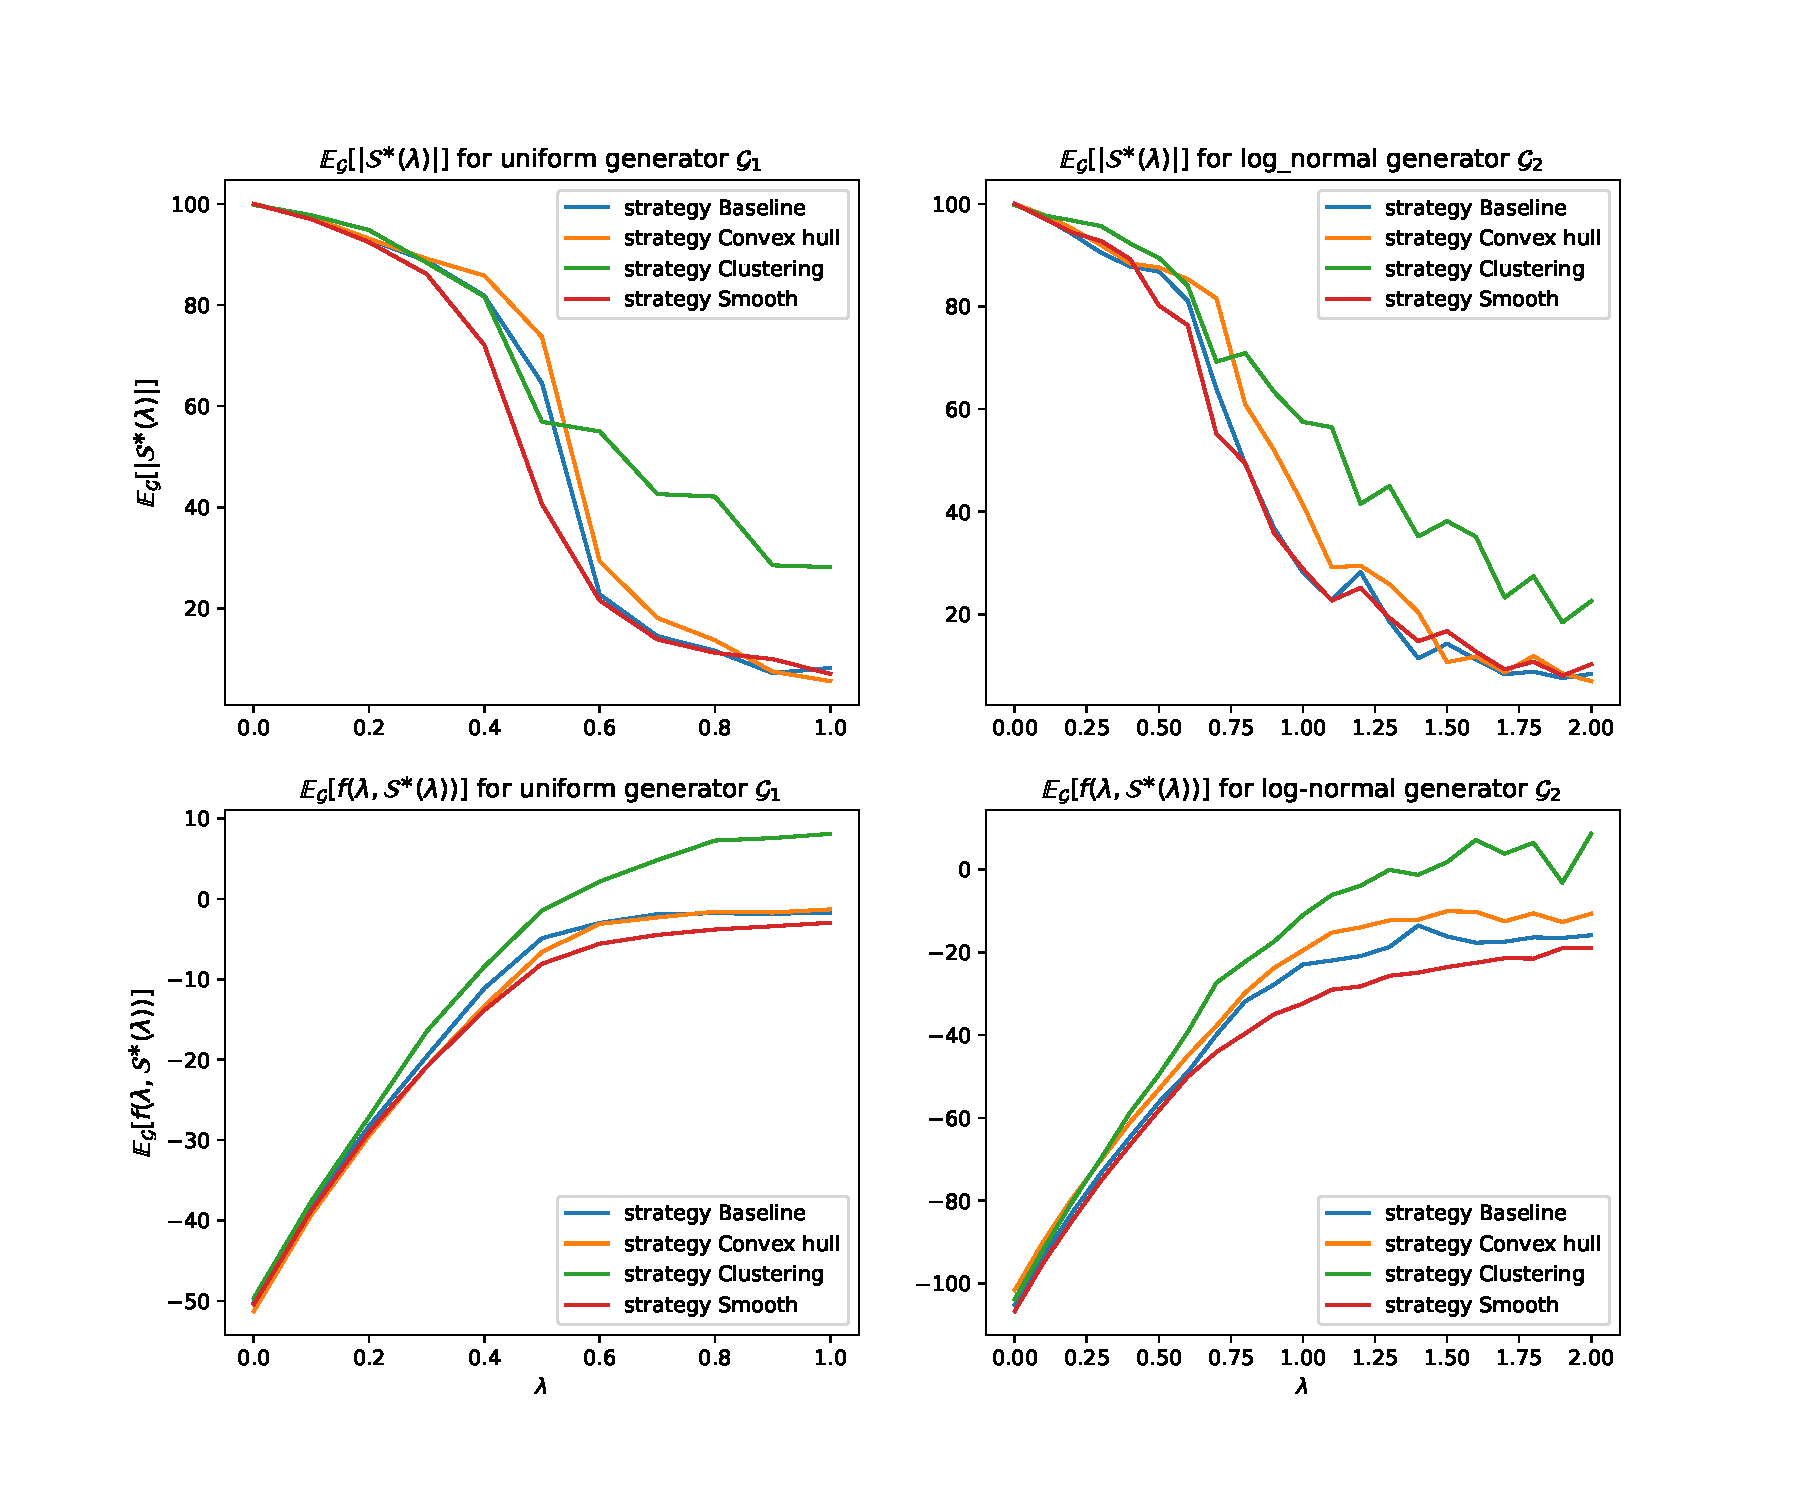
\includegraphics[width=\linewidth, trim=55 55 55 55, clip]{images/Expectation_f_num_cities_100.pdf}
    \caption{For all our techniques, we plot the expected number of cities being
    selected for both data sets $\mathcal{G}_1$ and $\mathcal{G}_2$ (top) over
    different values of $\lambda$. We also plot the expected loss value as we
    change $\lambda$ (bottom). All results have been averaged over 20 different
    random seeds. the total number of cities was $100$ in this experiment. Our
    continuous Markov chain (here called "Smooth") consistently outperforms all our other
    implementations.}
    \label{fig:loss_plots100}
\end{figure}


\begin{figure}
    \centering
    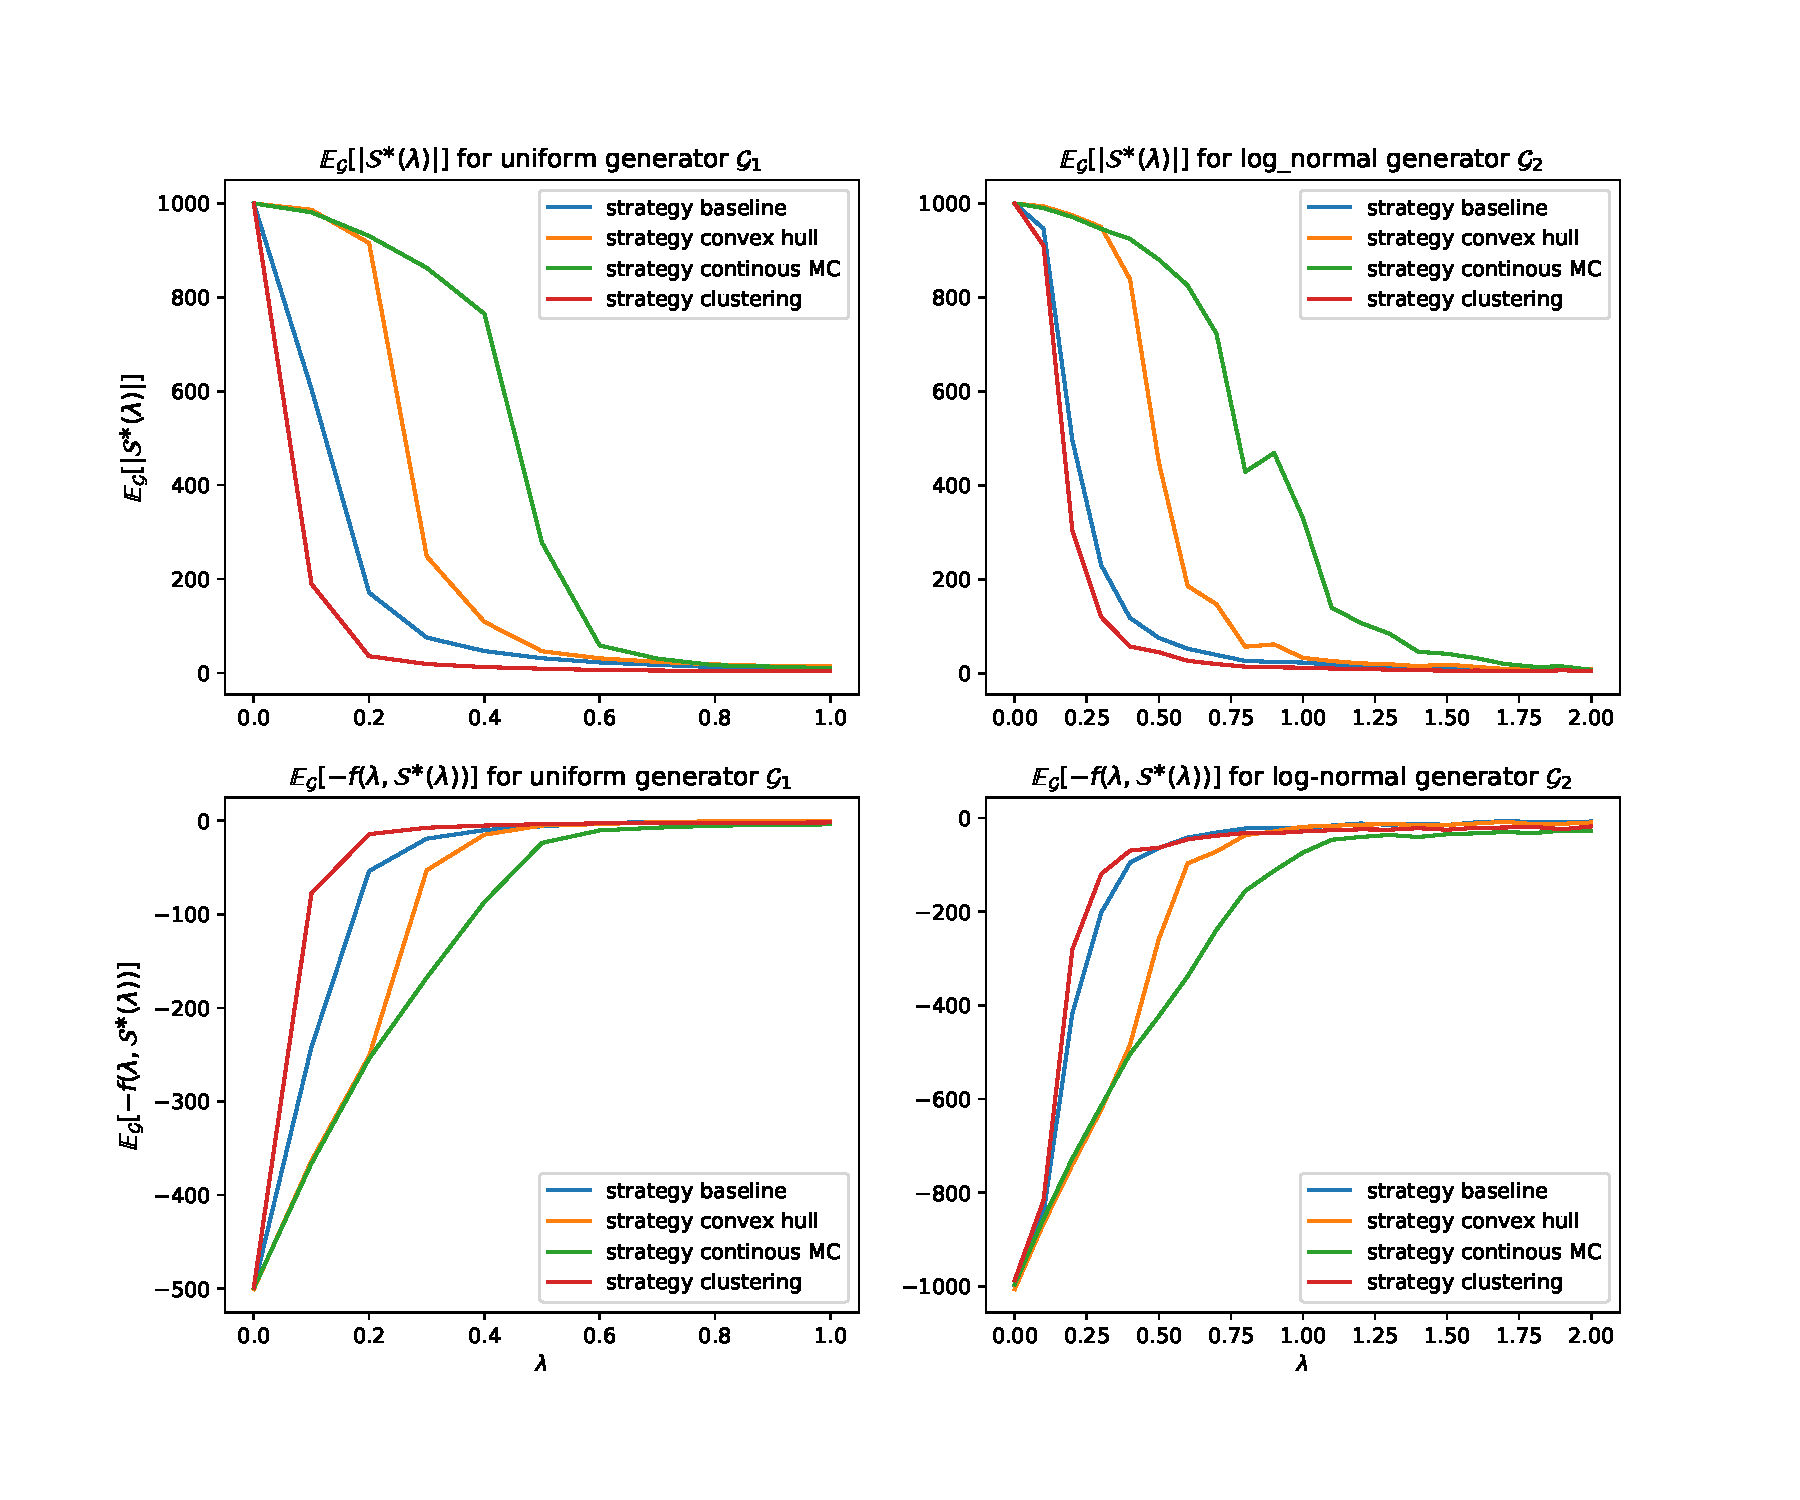
\includegraphics[width=\linewidth, trim=55 55 55 55, clip]{images/Expectation_f_num_cities_1000.pdf}
    \caption{We plot the number of selected cities and expected loss values also for $n=1000$. Again, our continuous Markov chain outperforms the other techniques (the names and ordering of techniques are different from Figure~\ref{fig:loss_plots100} since we did not have time to regenerate this result. }
    \label{fig:loss_plots}
\end{figure}

\begin{figure}
    \centering
    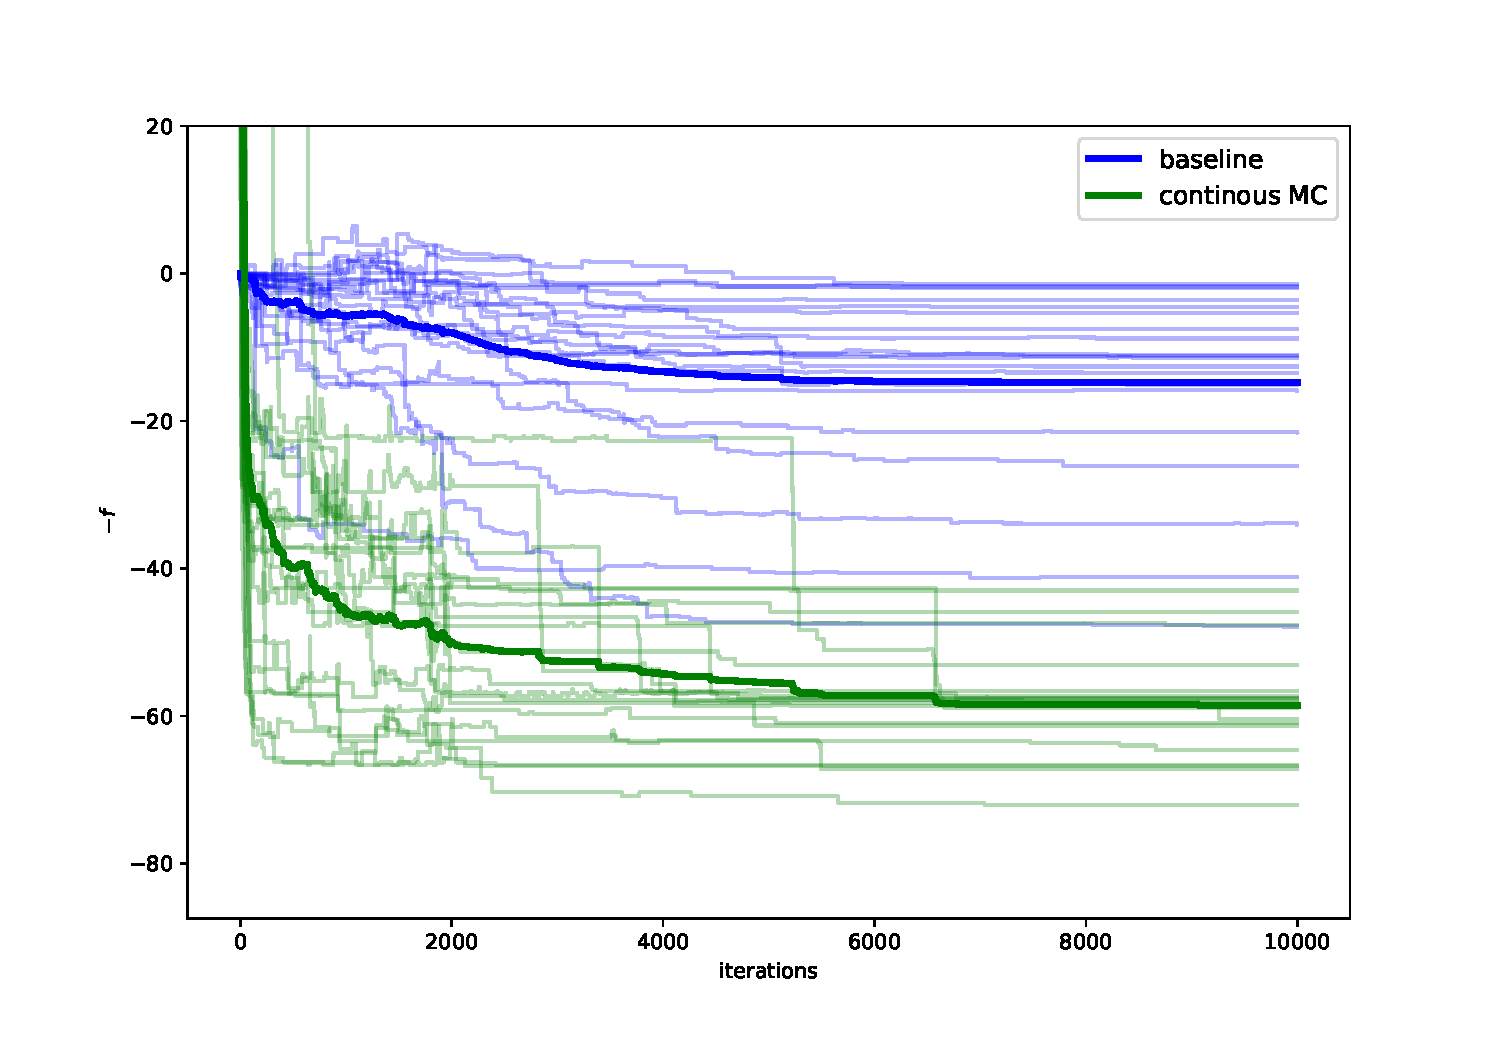
\includegraphics[width=\linewidth]{images/stability.pdf}
    \caption{Stability of the continuous Markov Chain strategy. The thin light-colored lines show each of the 20 runs of the algorithm with different initializations. The bold dark-colored lines show the average over all runs.}
    \label{fig:stability}
\end{figure}

\subsection{Stability}
Another favorable feature of the continuous Markov Chain strategy is that it is
less susceptible to the random initialization compared to the other strategies.
Figure \ref{fig:stability} shows that the baseline strategy can perform
drastically different depending on the random seed, whereas the continuous
Markov Chain strategy is more stable and shows less deviation in the minimum
loss value it can reach. Note that occasionally the baseline strategy will
produce good results, but just not reliably.

\section{Conclusion}
We explored the Metropolis algorithm to optimize a complex geometric objective
function which is highly non-convex. We found that the transition strategy
between the states has a significant influence on the performance of the
Metropolis algorithm on optimizing this objective function. Mainly we observed
that for a large number of cities, the strategies which only add or remove one
city in each iteration are slow and usually struggle to find an optimal set of
cities which is far from the initial cities selected in the first iterations. In
light of this observation, we proposed to use a continuous Markov Chain to move
between the states as our best strategy. We claim that this strategy helps to
explore the whole map of cities more efficiently to find the optimal set of
cities. The solution set derived by this method are always circular, but in
practice they can be used as an initialization to the baseline method to find a
more optimal solution. Overall, we believe that our method strikes a good
balance between quality of results and computation time.


\bibliographystyle{IEEEtran}
\bibliography{literature}

\end{document}
